%%%%%%%%%%%%%%%%%%%%%%%%%%%%%%%%%%%%%%%%%%%%%%%%%%%%%%%%%%%%%%%%%
% Tese de Doutorado / Dept Fisica, CFM, UFSC                    %
% Andre@UFSC - 2014                                             %
%%%%%%%%%%%%%%%%%%%%%%%%%%%%%%%%%%%%%%%%%%%%%%%%%%%%%%%%%%%%%%%%%

%:::::::::::::::::::::::::::::::::::::::::::::::::::::::::::::::%
%                                                               %
%                          Capítulo 1                           %
%                                                               %
%:::::::::::::::::::::::::::::::::::::::::::::::::::::::::::::::%

%***************************************************************%
%                                                               %
%                         Introdução                            %
%                                                               %
%***************************************************************%

\chapter{Introdução}
\label{sec:intro}

%***************************************************************%
%                                                               %
%                         Intro - IFS                           %
%                                                               %
%***************************************************************%

\section{Espectroscopia de campo integral}

Na última década presenciamos uma proliferação de surveys de imageamento e
espectroscopia. Surveys como o SDSS \citep{York2000}, ALHAMBRA \citep{Moles2008}
e COSMOS \citep{Scoville2007}, para citar alguns exemplos, permitem explorar a
distribuição espectral de energia (SED\footnote{\em Spectral Energy
Distribution.}) de centenas de milhares a milhões de galáxias.
Entretanto, da forma como estes surveys são executados, há sempre um compromisso
entre a resolução espacial e a espectral. As imagens obtidas pelo SDSS têm um
boa resolução espacial, mas mapeiam a SED de forma grosseira, com apenas $5$
filtros de banda larga ($ugriz$). Já os espectros obtidos pelo mesmo survey
possuem uma excelente resolução e cobertura espectral, mas obtém o espectro
integrado da região central das galáxias.

O melhor dos dois mundos pode ser alcançado com instrumentos que fazem
espectroscopia de campo integral (IFS\footnote{\em Integral Field
Spectroscopy.}). Instrumentos que realizam este tipo de espectroscopia consistem
em geral de um amontoado de fibras óticas, as quais alimentam um espectrógrafo
comum. Assim, depois de um processo relativamente complicado de redução de
dados, obtém-se espectros espacialmente resolvidos com uma boa resolução
espectral e espacial. O survey CALIFA ({\em Calar Alto Legacy Integral Field
Area survey\footnote{\url{http://www.caha.es/CALIFA/}}}) está utilizando o
instrumento PMAS/PPAK do observatório Calar Alto para obter IFS de $600$
galáxias \citep{Sanchez2012}.
Destas, $100$ já estão disponíveis no primeiro {\em Data Release}
\citep[DR1]{Husemann2013}, afirmando o caráter de legado deste
survey.\fixme(atualizar comentário sobre data releases)

Quando completado, o CALIFA terá obtido da ordem de $10^6$ espectros, quase o
mesmo que o SDSS. Porém, este não será apenas mais um survey espectroscópico. A
riqueza do CALIFA está nas informações espacialmente resolvidas, em uma amostra
representativa do universo local ($0.005 < z < 0.03$, limitada em diâmetro
angular) cobrindo a distribuição de galáxias no diagrama cor--magnitude da nuvem
azul à sequência vermelha, amostrando galáxias todos os tipos morfológicos
(espirais, elípticas, irregulares e até mesmo alguns sistemas em interação).

\begin{figure}
	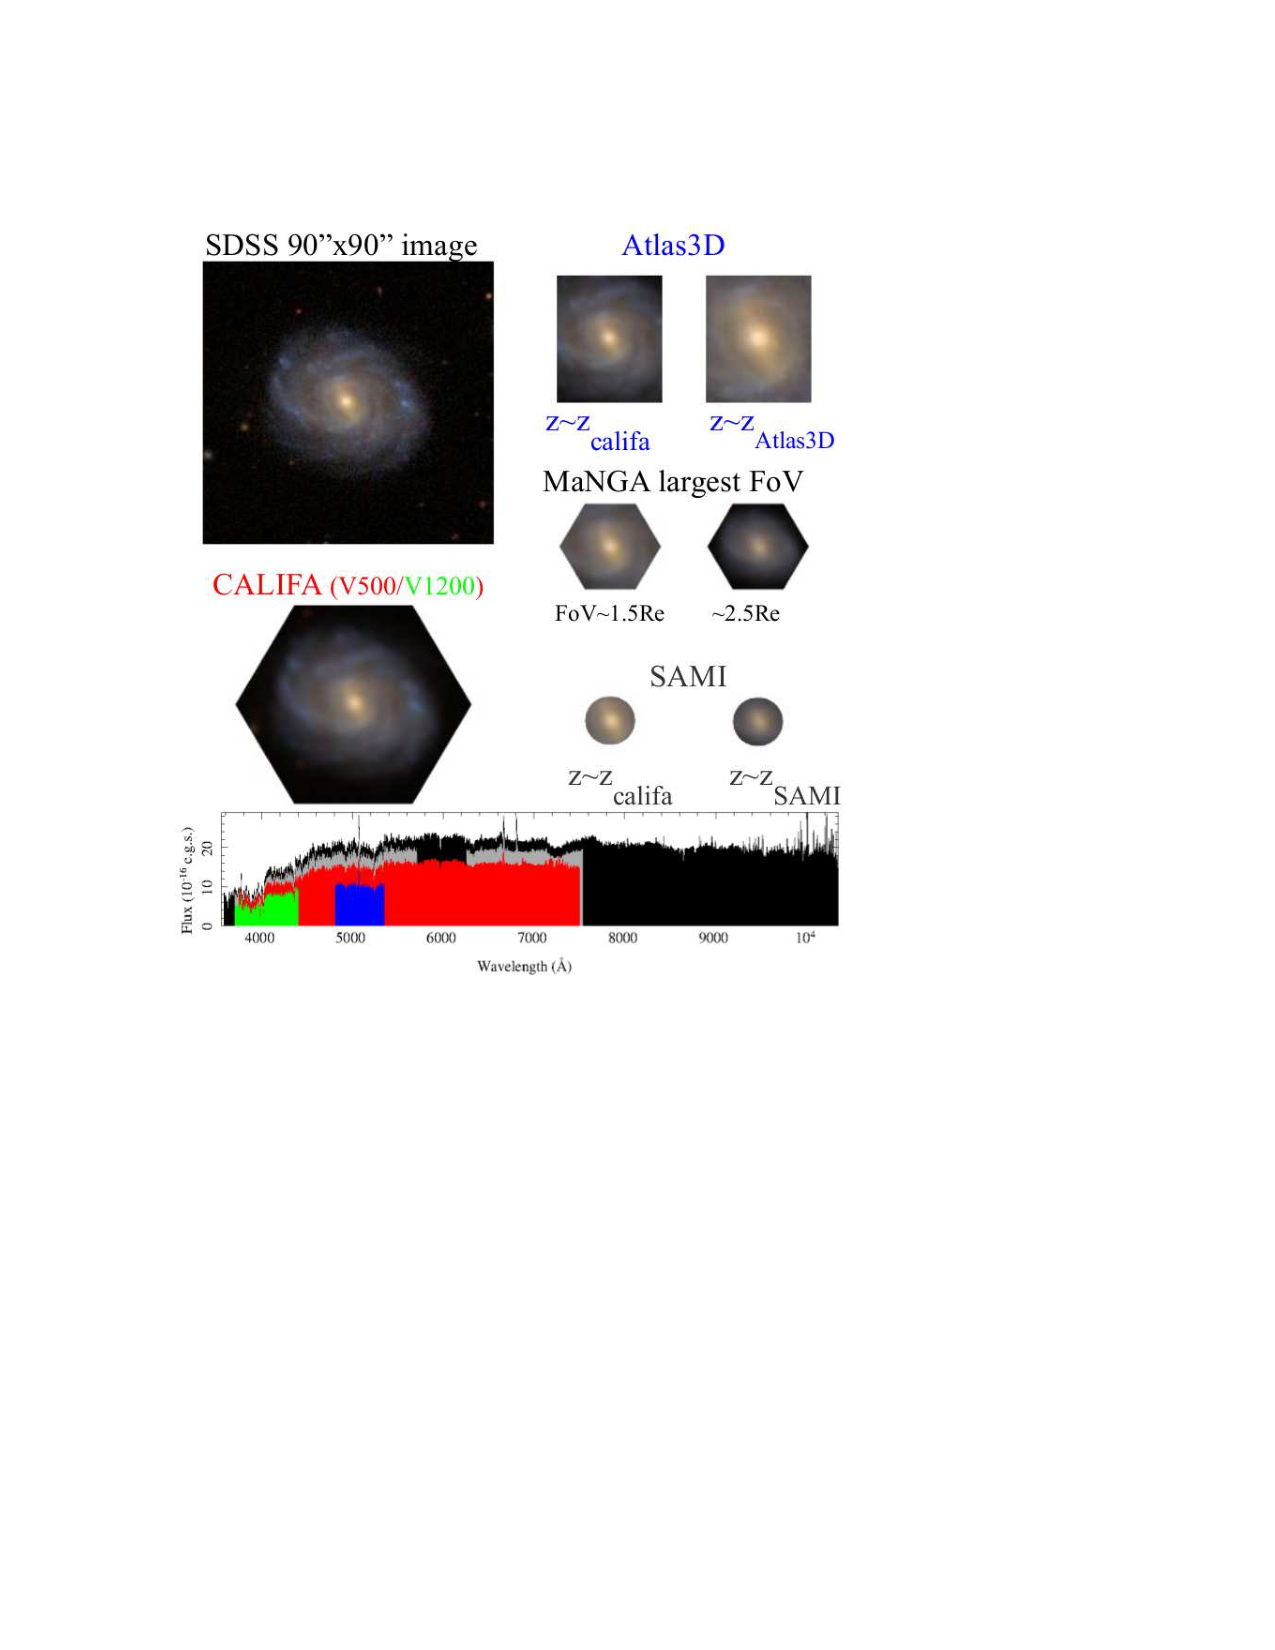
\includegraphics{figuras/surveysIFS}
	\caption[Comparação entre {\em surveys} espectroscópicos de campo integral.]
	{\TODO: Comparação entre {\em surveys} espectroscópicos de campo integral.
	Retirado de \citet{Sanchez2014}.}
	\label{fig:surveysIFS}
\end{figure}

Comparado a outros {\em surveys} já realizados, como o Altas3D
\citep{Cappellari2011} ou o {\em Disk Mass Survey} (DMS) \citep{Bershady2010}, o
CALIFA cobre uma faixa muito maior de tipos morfológicos e massas. Outros {\em
surveys} que estão em andamento são o SAMI \citep{Croom2012, Bryant2015} e o
MaNGA \citep{Bundy2015}. Estes também buscam obter uma amostra grande de
galáxias, até maior do que a do CALIFA. Entretanto, a vantagem do CALIFA está na
cobertura e amostragem espacial, observando uma maior porção de cada galáxia com
mais riqueza de detalhes. \TODO Falar da Figura \ref{fig:surveysIFS}, pegar
alguma coisa de \citet{Sanchez2014}.

%***************************************************************%
%                                                               %
%                Intro - Stellar synthesis of IFS               %
%                                                               %
%***************************************************************%

\section{Síntese de população estelar espacialmente resolvida}
\label{sec:Intro:Sintese}

Os espectros espacialmente resolvidos do CALIFA podem ser descritos como um cubo
de dados, com as duas primeiras dimensões sendo a posição $x$ e $y$ (ascensão
reta e declinação) e a terceira sendo o comprimento de onda. Nestes cubos,
planos com comprimento de onda constante são imagens, enquanto ``fatias''
definidas por um par $(x, y)$ constante são espectros. Pode-se tratar estes
espectros individualmente, embora na verdade, nos cubos do CALIFA os pixels
vizinhos estão correlacionados devido ao {\em seeing} do céu e ao processo de
observação. Há a queda na relação sinal/ruído (S/N) nas regiões mais afastadas
do núcleo da galáxia, onde o brilho superficial é muito menor.
Algumas galáxias possuem outros objetos ``intrusos'' que precisam ser
mascarados. Linhas telúricas\footnote{Linhas de absorção causadas pela
atmosfera.} também precisam ser mascaradas. Assim, em geral, é necessário um
preprocessamento visando manter um S/N mínimo e garantir um espectro livre de
contaminação. Os detalhes sobre o preprocessamento utilizado neste trabalho
estão descritos na seção 3 do Apêndice \ref{apendice:PaperResolving1}.

Um aspecto importante do preprocessamento utilizado é que o cubo de dados é
dividido em zonas de Voronoi, onde regiões com baixo S/N são combinadas formando
efetivamente ``pixels maiores''. Desta forma, o cubo original é transformado
numa matriz de zonas e comprimento de onda, onde fatias de zona constante são
espectros. Com isso, os espectros, e as máscaras e erros que os acompanham,
estão prontos para serem usados pelo próximo passo.

A síntese de população estelar consiste em obter a história de formação estelar
(SFH) de uma galáxia utilizando modelos de população estelar simples (SSP).
Ajusta-se o espectro de uma galáxia como a soma de espectros de SSPs com idades
e composições químicas distintas (levando em conta a atenuação por poeira). O
resultado é um vetor de frações de luz e massa destas SSPs, que podem ser
facilmente convertidos a uma SFH conforme a prescrição de \cite{Asari2007}.
O programa utilizado é o \starlight, desenvolvido por \cite{CidFernandes2005}.

Passamos todos os espectros das zonas pelo \starlight, obtendo o resultado da
síntese como um arquivo de síntese separado para cada zona. Entretanto, para
visualizar ou mesmo tentar entender estes resultados, é preciso organizar e
converter estes arquivos para um formato mais adequado.


%***************************************************************%
%                                                               %
%                        Intro - PyCASSO                        %
%                                                               %
%***************************************************************%

\section{O nascimento do PyCASSO}

Todo o descrito anteriormente forma o alicerce deste presente trabalho. Porém,
dada a grande quantidade de dados espalhados em diversos formatos, a análise dos
resultados da síntese de populações estelares para uma determinada galáxia pode
se tornar um grande e complexo quebra-cabeças computacional. Trabalhar com todas
as galáxias do {\em survey} fica virtualmente impossível desta forma. Assim, da
necessidade de manipular os resultados da síntese dos cubos de dados das
galáxias do CALIFA, nasceu o software PyCASSO.

PyCASSO ({\em Python CALIFA \starlight Synthesis Organizer}) é um software
desenvolvido em Python com o objetivo de organizar gerenciar os dados produzidos
pelo \starlight com base nos dados do CALIFA. O survey CALIFA é apresentado no
Capítulo \ref{sec:ifs}, que também discute os softwares QBICK e \starlight,
ferramentas básicas em nossa análise doe cubos de dados. O Capítulo
\ref{sec:pycasso} apresenta a documentação do PyCASSO, e em seguida discute os
artigos publicados que o utilizam intensivamente.


%***************************************************************%
%                                                               %
%                      Intro - Decomposicao                     %
%                                                               %
%***************************************************************%

\section{Decomposição morfológica de galáxias}

\TODO detalhar mais aqui, ainda não tá legal. O Capitulo \ref{sec:morph}
apresenta um beabá sobre morfologia.

\TODO Caracterização ds PSF no Capítulo \ref{sec:psf}. Explicar a importância
de fazer isso pro survey.

Como aplicação científica do PyCASSO, o Capítulo \ref{sec:pop} trata da síntese
espectral das componentes morfológicas (bojo e disco) de uma galáxia, obtidas no
conforme foi descrito no Capítulo \ref{sec:Decomp}. Estas componentes são
armazenadas em cubos de dados, e são tratados exatamente da mesma forma que
uma galáxia. Seus espectros são passados pelo \starlight, resultando em cubos
de síntese espectral. Os dados da síntese das componentes foram comparados com a
síntese da galáxia original, utilizando o programa PyCASSO. \TODO O que
resultou?


% End of this chapter
